\chapter{El aire, una mezcla de gases}\label{ch:g4:air-a-mixture-of-gases}

Un día de viento, una cometa tira de su cuerda y, en el lago, una vela
se hincha y empuja una barca. Algo las empuja, y sin embargo no se ve
nada. Ese algo es el \omterm{def:g4:air-a-mixture-of-gases:air}{aire}. No podemos verlo, pero está a nuestro
alrededor, llena cada botella vacía y cada habitación, y lo tomamos en
cada respiración. ¿De qué está hecho el \omterm{def:g4:air-a-mixture-of-gases:air}{aire}?

\begin{recall}
\omterm{def:g2:mixing-and-dissolving:mix}{Mezclar} es juntar cosas distintas; lo que obtenemos es una mezcla de
esas cosas, y al mezclarlas no se pierde nada
(\cref{ch:g2:mixing-and-dissolving}).
\end{recall}

\begin{omfigure}
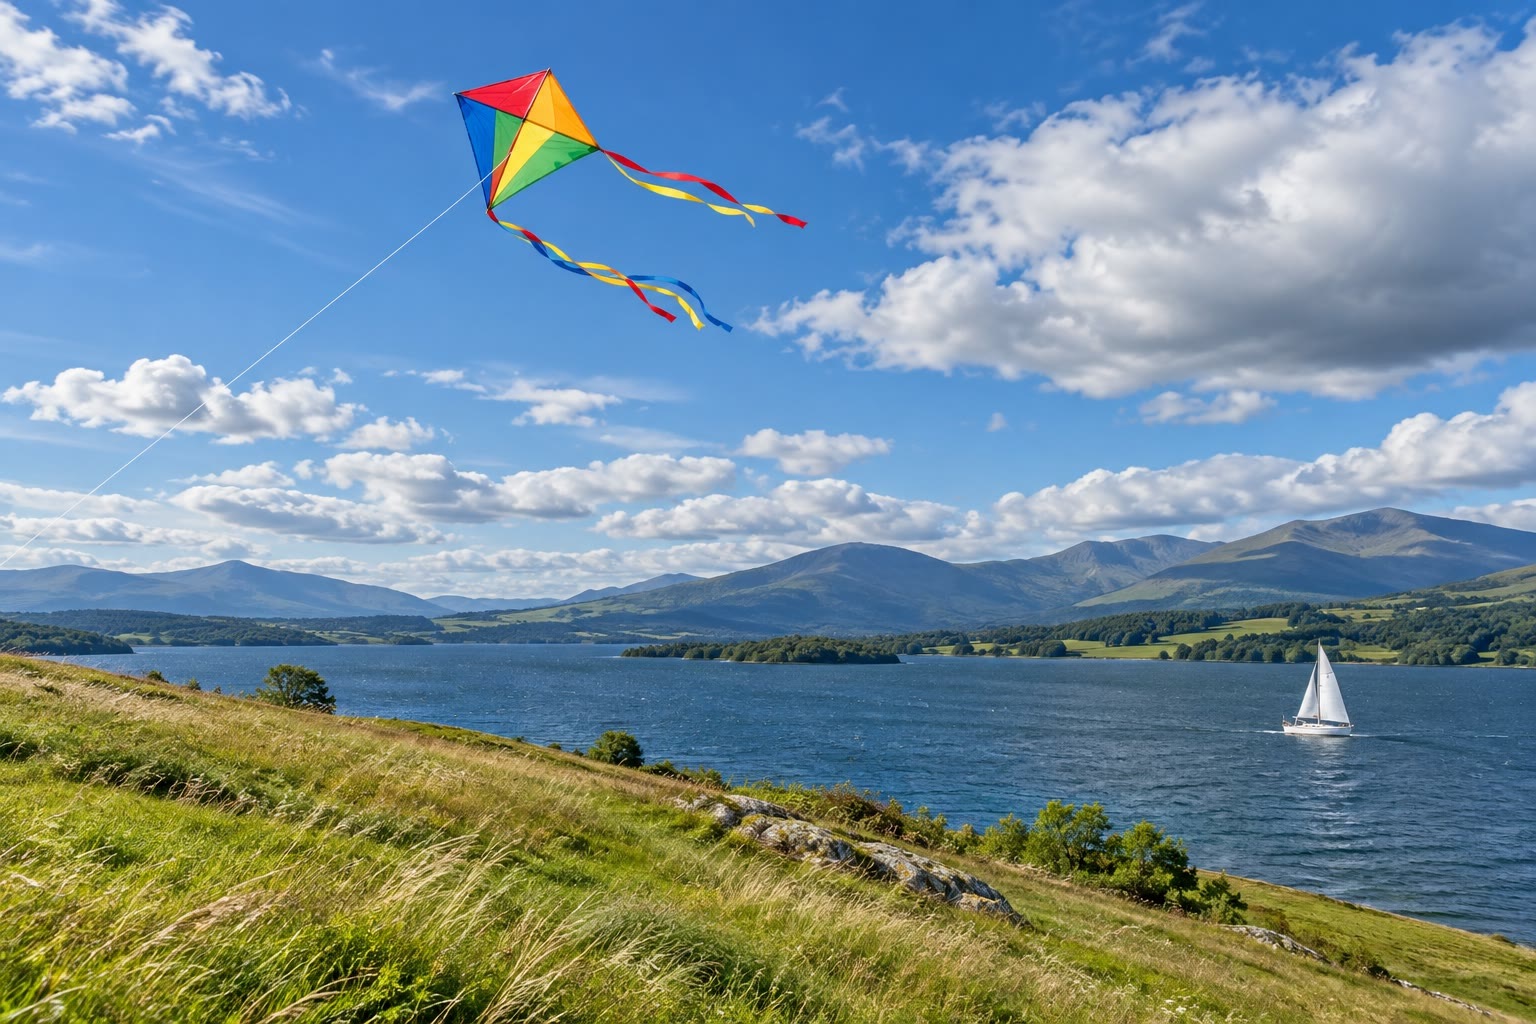
\includegraphics[width=0.6\linewidth]{images/book1/ai/g4-kite-day.jpg}

{\small Una cometa y una vela: el \omterm{def:g4:air-a-mixture-of-gases:air}{aire} no se ve, pero empuja.}
\end{omfigure}

\section{El aire está a nuestro alrededor}

\begin{example}[Un vaso boca abajo]\label{ex:g4:air-a-mixture-of-gases:glass}
Metemos un pañuelo de papel seco en el fondo de un vaso vacío. Damos la
vuelta al vaso y lo hundimos recto en un cuenco con agua. Cuando lo
sacamos, el pañuelo sigue seco. El vaso no estaba vacío: estaba lleno de
\omterm{def:g4:air-a-mixture-of-gases:air}{aire}, y el \omterm{def:g4:air-a-mixture-of-gases:air}{aire} impedía que entrara el agua.
\end{example}

\begin{omfigure}
\begin{tikzpicture}[font=\small, scale=1.3]
  \pic[transform shape] at (0,0) {trough};
  % the upturned glass, rim at y = 0.35, base at y = 2.35
  \fill[white] (-0.8,0.5) rectangle (0.8,0.95);
  \pic[transform shape, rotate=180] at (0,2.35) {beaker={0}{white}};
  % the tissue at the top, inside
  \fill[white, draw=black!45, rounded corners=1.5pt] (-0.4,2.33) -- (-0.3,2.05)
    -- (-0.1,2.12) -- (0.05,1.98) -- (0.25,2.1) -- (0.42,2.02) -- (0.45,2.33) -- cycle;
  \draw[<-, omProp, thick] (0.45,2.12) -- (2.4,2.5) node[right, text=black]
    {un pañuelo seco};
  \draw[<-, omProp, thick] (0.3,1.2) -- (2.4,1.4) node[right, text=black]
    {aire: impide que entre el agua};
  \draw[<-, omProp, thick] (1.4,0.7) -- (2.4,0.55) node[right, text=black]
    {agua};
\end{tikzpicture}

{\small Hundimos el vaso boca abajo en el agua. El \omterm{def:g4:air-a-mixture-of-gases:air}{aire} atrapado dentro
impide que entre el agua, y el pañuelo sigue seco.}
\end{omfigure}


\begin{remark}[El aire es un gas]\label{rem:g4:air-a-mixture-of-gases:gas}
El \omterm{def:g4:air-a-mixture-of-gases:air}{aire} es un gas: no tiene forma propia y se extiende hasta llenar
cualquier recipiente. Aun así es materia, y un globo lleno de \omterm{def:g4:air-a-mixture-of-gases:air}{aire} pesa
un poco más que el mismo globo vacío. Qué son los gases, y por qué se
comportan así, lo cuenta el libro de física.
\end{remark}

\section{El aire es una mezcla}

\begin{definition}[Aire]\label{def:g4:air-a-mixture-of-gases:air}
El \emph{aire}\index{aire} es la mezcla de gases que rodea la Tierra.
No es un único gas: en él hay varios gases \omterm{def:g2:mixing-and-dissolving:mix}{mezclados}, que se pueden
separar unos de otros.
\end{definition}

\begin{proposition}[De qué está hecho el aire]\label{prop:g4:air-a-mixture-of-gases:composition}
% ledger: air:N2, air:O2, air:Ar, air:trace, air:CO2, air:H2O
Sin contar su vapor de agua, el \omterm{def:g4:air-a-mixture-of-gases:air}{aire} está formado por:
\begin{itemize}
  \item \textbf{nitrógeno}, unas cuatro quintas partes del \omterm{def:g4:air-a-mixture-of-gases:air}{aire};
  \item \textbf{oxígeno}, más o menos una quinta parte del \omterm{def:g4:air-a-mixture-of-gases:air}{aire};
  \item un poco de \textbf{argón}, alrededor de 1 parte de cada 100;
  \item muy poco \textbf{dióxido de carbono}, unas 4 partes de cada
        10\,000, y cantidades diminutas de otros gases.
\end{itemize}
El \omterm{def:g4:air-a-mixture-of-gases:air}{aire} contiene también \textbf{vapor de agua}, invisible: muy poco en
un día frío y seco, y hasta unas 4 partes de cada 100 en un día cálido y
húmedo.
\end{proposition}

\begin{example}[Cien botellas de aire]\label{ex:g4:air-a-mixture-of-gases:hundred}
% ledger: air:N2, air:O2, air:Ar
Imagina 100 botellas de \omterm{def:g4:air-a-mixture-of-gases:air}{aire} seco, con los gases del \omterm{def:g4:air-a-mixture-of-gases:air}{aire} repartidos en
botellas separadas. Unas 78 botellas contendrían nitrógeno, 21 botellas
oxígeno y la última botella argón, con unas gotitas de dióxido de
carbono y de otros gases.
\end{example}

\begin{omfigure}
\begin{tikzpicture}[font=\small, x=0.42cm, y=0.42cm]
  \foreach \k in {0,...,99} {
    \pgfmathtruncatemacro\col{mod(\k,10)}
    \pgfmathtruncatemacro\row{9-int(\k/10)}
    \ifnum\k<78 \def\c{omDef!45}\else\ifnum\k<99 \def\c{red!45}\else\def\c{cyan!60}\fi\fi
    \fill[\c, draw=white, line width=0.8pt] (\col,\row) rectangle ++(1,1);
  }
  \fill[omDef!45] (12,8) rectangle ++(1,1);
  \node[anchor=west] at (13.3,8.5) {nitrógeno: 78 cuadrados};
  \fill[red!45] (12,6) rectangle ++(1,1);
  \node[anchor=west] at (13.3,6.5) {oxígeno: 21 cuadrados};
  \fill[cyan!60] (12,4) rectangle ++(1,1);
  \node[anchor=west, align=left] at (13.3,4.5) {argón, dióxido de carbono\\ y el resto: 1 cuadrado};
\end{tikzpicture}

{\small Cien cuadrados de \omterm{def:g4:air-a-mixture-of-gases:air}{aire} seco. El cuadrado de abajo a la derecha
contiene el argón y el dióxido de carbono, demasiado pequeño para
dibujarlo aparte.}
\end{omfigure}

\begin{remark}[Nombres de gases]\label{rem:g4:air-a-mixture-of-gases:names}
Nitrógeno, oxígeno, argón y dióxido de carbono son nombres de gases.
Todos son incoloros y no tienen olor. Un capítulo posterior muestra de
qué está hecho cada uno, hasta llegar a las piezas diminutas que forman
toda la materia.
\end{remark}

\section{Lo que inspiramos y lo que espiramos}

\begin{proposition}[El aire espirado]\label{prop:g4:air-a-mixture-of-gases:breath}
% ledger: breath:O2, breath:CO2, breath:N2, air:O2, air:CO2
El \omterm{def:g4:air-a-mixture-of-gases:air}{aire} que espiramos no es el \omterm{def:g4:air-a-mixture-of-gases:air}{aire} que inspiramos. Nuestro cuerpo toma
parte del oxígeno y desprende dióxido de carbono y vapor de agua:
\begin{itemize}
  \item unas 21 partes de cada 100 del \omterm{def:g4:air-a-mixture-of-gases:air}{aire} inspirado son oxígeno, pero
        solo unas 16 partes de cada 100 del \omterm{def:g4:air-a-mixture-of-gases:air}{aire} espirado;
  \item el dióxido de carbono pasa de unas 4 partes de cada 10\,000 a
        unas 4 partes de cada 100: unas cien veces más;
  \item el nitrógeno se espira tal como se inspiró.
\end{itemize}
\end{proposition}

\begin{omfigure}
\begin{tikzpicture}
\begin{axis}[ybar, width=0.8\linewidth, height=5.2cm, bar width=12pt,
    ymin=0, ymax=90, ylabel={partes de cada 100},
    symbolic x coords={nitrogen, oxygen, carbon dioxide}, xtick=data,
    xticklabels={nitrógeno, oxígeno, dióxido de carbono},
    tick label style={font=\small}, label style={font=\small},
    xticklabel style={text height=1.6ex, text depth=0.4ex},
    legend style={font=\small, at={(0.98,0.95)}, anchor=north east},
    nodes near coords, nodes near coords style={font=\footnotesize},
    enlarge x limits=0.25, axis lines*=left, ymajorgrids,
    grid style={gray!20}]
% ledger: air:N2, air:O2, air:CO2, breath:N2, breath:O2, breath:CO2 (rounded)
\addplot[fill=omDef!45, draw=omDef] coordinates
  {(nitrogen,78) (oxygen,21) (carbon dioxide,0)};
\addplot[fill=omProp!55, draw=omProp] coordinates
  {(nitrogen,78) (oxygen,16) (carbon dioxide,4)};
\legend{inspirado, espirado}
\end{axis}
\end{tikzpicture}

{\small \omterm{def:g4:air-a-mixture-of-gases:air}{Aire} inspirado y \omterm{def:g4:air-a-mixture-of-gases:air}{aire} espirado, en partes de cada 100 (sin contar
el vapor de agua; cifras redondeadas). El dióxido de carbono del \omterm{def:g4:air-a-mixture-of-gases:air}{aire}
inspirado, 4 partes de cada 10\,000, es demasiado poco para verse como
barra.}
\end{omfigure}

\begin{example}[Una habitación llena de gente]\label{ex:g4:air-a-mixture-of-gases:room}
En un aula pequeña con las ventanas cerradas, treinta personas espiran
dióxido de carbono durante toda la mañana. Poco a poco, el \omterm{def:g4:air-a-mixture-of-gases:air}{aire} del aula
contiene menos oxígeno y más dióxido de carbono, y la gente se siente
cansada. Al abrir las ventanas vuelve a entrar \omterm{def:g4:air-a-mixture-of-gases:air}{aire} fresco.
\end{example}

\begin{omfigure}
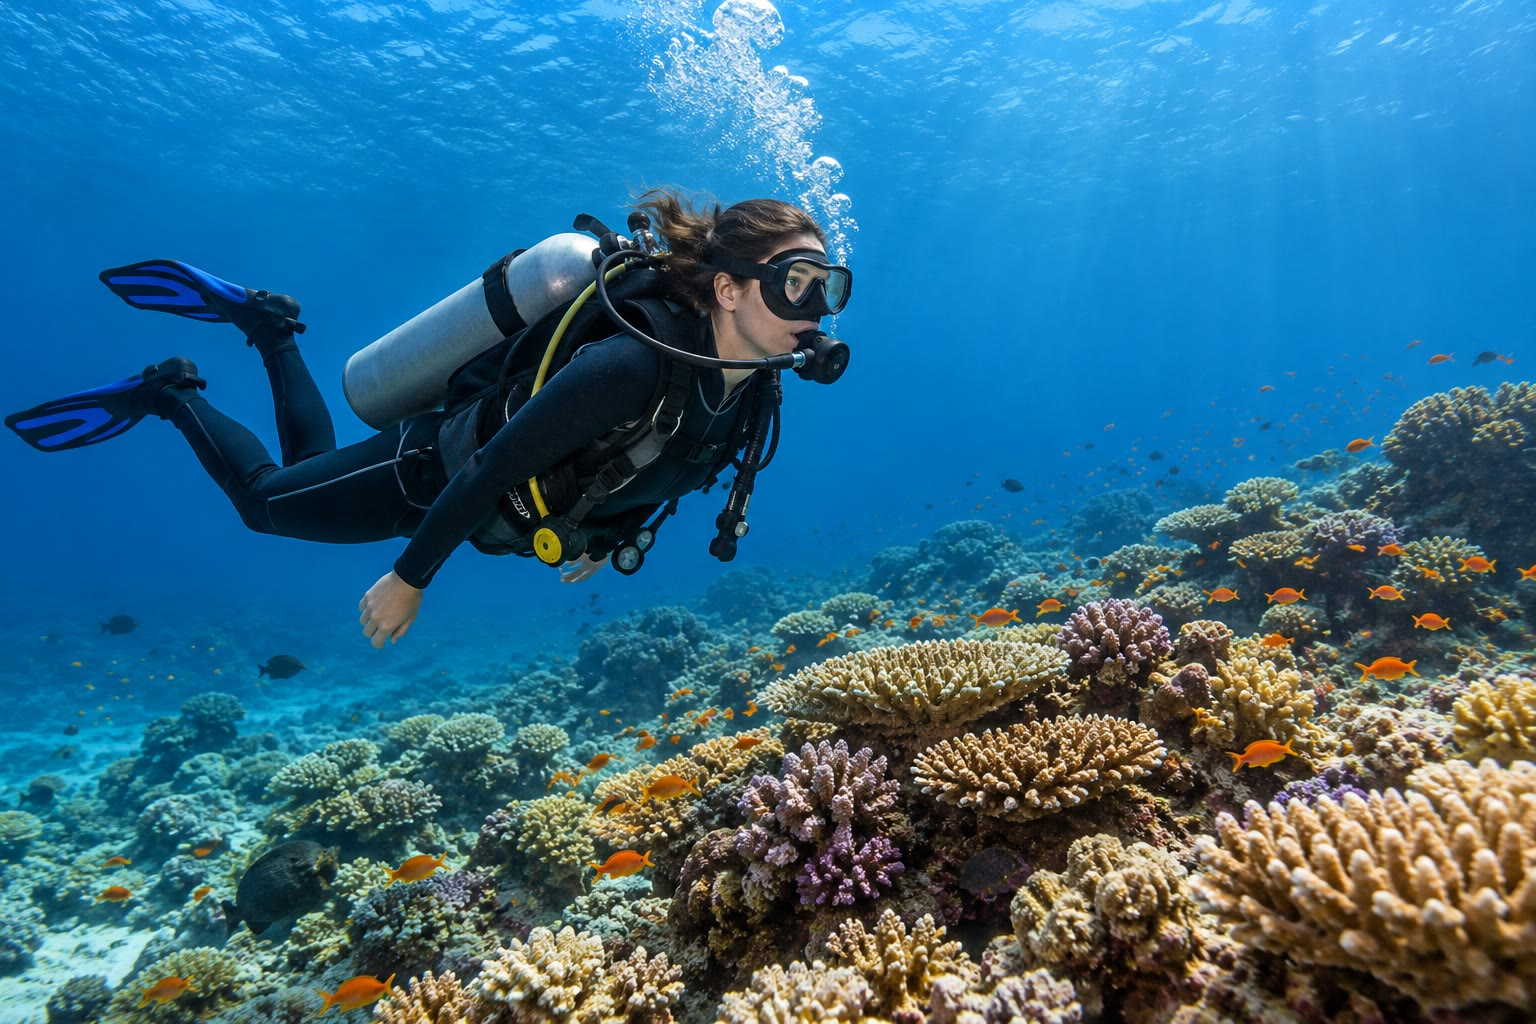
\includegraphics[width=0.55\linewidth]{images/book1/ai/g4-scuba-diver.jpg}

{\small Un buceador respira el \omterm{def:g4:air-a-mixture-of-gases:air}{aire} de la botella que lleva a la espalda;
las burbujas son el \omterm{def:g4:air-a-mixture-of-gases:air}{aire} espirado.}
\end{omfigure}

\begin{remark}[Por qué los buceadores respiran aire]\label{rem:g4:air-a-mixture-of-gases:diver}
La botella de un buceador está llena de \omterm{def:g4:air-a-mixture-of-gases:air}{aire} comprimido en un espacio
pequeño, no de oxígeno puro: respirar oxígeno puro a mucha profundidad
es peligroso. El nitrógeno del \omterm{def:g4:air-a-mixture-of-gases:air}{aire} está ahí para diluir el oxígeno.
\end{remark}

\section{Oxígeno para la vida y para el fuego}

\begin{proposition}[Los seres vivos y las llamas gastan oxígeno]\label{prop:g4:air-a-mixture-of-gases:oxygen}
De todos los gases del \omterm{def:g4:air-a-mixture-of-gases:air}{aire}, el oxígeno es el que necesitan los seres
vivos y las llamas. Los animales y las personas lo toman al respirar;
una llama lo toma del \omterm{def:g4:air-a-mixture-of-gases:air}{aire} que la rodea. Las plantas verdes, con la luz
del día, devuelven oxígeno al \omterm{def:g4:air-a-mixture-of-gases:air}{aire}.
\end{proposition}

\begin{inthelab}[Una vela bajo un tarro]
El profesor enciende una vela sobre un azulejo y baja despacio sobre
ella un tarro grande de vidrio. La llama se encoge, parpadea y se apaga
al cabo de unos segundos: alrededor de la llama, el \omterm{def:g4:air-a-mixture-of-gases:air}{aire} contiene
demasiado poco oxígeno para que siga ardiendo. Bajo un tarro el doble
de grande, la vela arde más o menos el doble de tiempo, porque hay más o
menos el doble de \omterm{def:g4:air-a-mixture-of-gases:air}{aire}, y por tanto el doble de oxígeno, para gastar.
\end{inthelab}

\begin{omfigure}
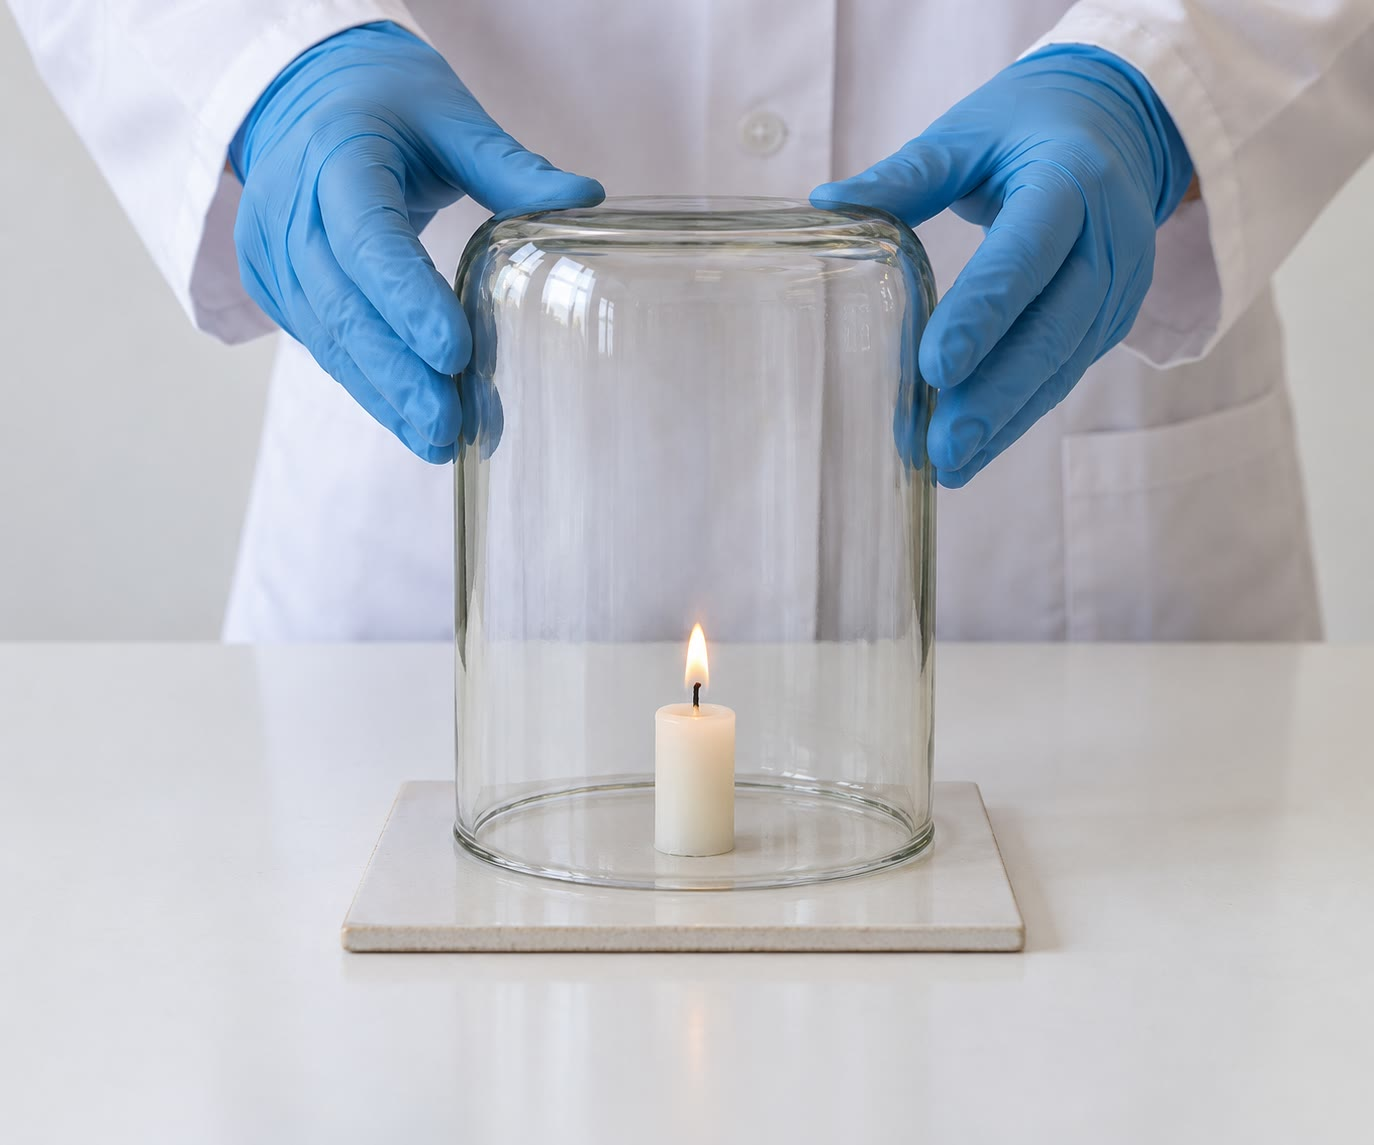
\includegraphics[width=0.5\linewidth]{images/book1/ai/g4-candle-jar-lab.jpg}

{\small Una vela bajo un tarro de vidrio se apaga cuando queda demasiado
poco oxígeno alrededor de su llama.}
\end{omfigure}

\begin{remark}[El nitrógeno no arde]\label{rem:g4:air-a-mixture-of-gases:nitrogen}
El nitrógeno es la mayor parte del \omterm{def:g4:air-a-mixture-of-gases:air}{aire} y, sin embargo, no mantiene
encendida una llama ni lo usa nuestro cuerpo. Si el \omterm{def:g4:air-a-mixture-of-gases:air}{aire} fuera todo
nitrógeno, no podríamos respirar y nada podría arder.
\end{remark}

\section{Ejercicios}

\begin{exercise}[$\star$]\label{exo:g4:air-a-mixture-of-gases:1}
¿El \omterm{def:g4:air-a-mixture-of-gases:air}{aire} es un único gas o una mezcla? Nombra los dos gases principales
del \omterm{def:g4:air-a-mixture-of-gases:air}{aire}.
\end{exercise}

\begin{exercise}[$\star$]\label{exo:g4:air-a-mixture-of-gases:2}
¿Qué fracción del \omterm{def:g4:air-a-mixture-of-gases:air}{aire}, más o menos, es nitrógeno? ¿Qué fracción, más o
menos, es oxígeno?
\end{exercise}

\begin{exercise}[$\star$]\label{exo:g4:air-a-mixture-of-gases:3}
En 100 litros de \omterm{def:g4:air-a-mixture-of-gases:air}{aire} seco, ¿cuántos litros son nitrógeno, más o menos?
¿Y cuántos son oxígeno?
\end{exercise}

\begin{exercise}[$\star$]\label{exo:g4:air-a-mixture-of-gases:4}
Metemos una botella vacía boca abajo en un barreño con agua. ¿Por qué
el agua no llena la botella?
\end{exercise}

\begin{exercise}[$\star$]\label{exo:g4:air-a-mixture-of-gases:5}
Mira el diagrama de barras. ¿De qué gas hay menos en el \omterm{def:g4:air-a-mixture-of-gases:air}{aire} espirado?
¿De qué gas hay más?
\end{exercise}

\begin{exercise}[$\star$]\label{exo:g4:air-a-mixture-of-gases:6}
¿Qué gas del \omterm{def:g4:air-a-mixture-of-gases:air}{aire} necesita una llama? ¿Qué gas del \omterm{def:g4:air-a-mixture-of-gases:air}{aire} necesitamos
nosotros para respirar?
\end{exercise}

\begin{exercise}[$\star$]\label{exo:g4:air-a-mixture-of-gases:7}
Mira la figura de los 100 cuadrados. ¿Cuántos cuadrados son nitrógeno?
¿Cuántos no lo son?
\end{exercise}

\begin{exercise}[$\star$]\label{exo:g4:air-a-mixture-of-gases:8}
¿Por qué una vela bajo un tarro se apaga al cabo de un rato?
\end{exercise}

\begin{exercise}[$\star$]\label{exo:g4:air-a-mixture-of-gases:9}
En 500 litros de \omterm{def:g4:air-a-mixture-of-gases:air}{aire}, ¿cuántos litros son oxígeno, más o menos? (Una
quinta parte del \omterm{def:g4:air-a-mixture-of-gases:air}{aire} es oxígeno.)
\end{exercise}

\begin{exercise}[$\star\star$]\label{exo:g4:air-a-mixture-of-gases:10}
¿Por qué es buena idea abrir las ventanas del aula entre una clase y
otra?
\end{exercise}

\begin{exercise}[$\star\star$]\label{exo:g4:air-a-mixture-of-gases:11}
Una vela arde 10 segundos bajo un tarro pequeño. ¿Cuánto tiempo, más o
menos, ardería bajo un tarro que contuviera el triple de \omterm{def:g4:air-a-mixture-of-gases:air}{aire}?
\end{exercise}
